\documentclass{ctexart}

\author{李约瀚 \\ 14130140331 \\ qinka@live.com \\ qinka@qinka.pw}
\title{FPGA设计基础实验报告 (三)}

\usepackage{listings}
\usepackage[figuresright]{rotating}
\lstset{breaklines}

\begin{document}
    
        % Cover
        \thispagestyle{empty}
        \begin{center}
            \vspace*{4em}
            {\Huge\textbf{FPGA设计基础实验报告\\\vspace*{0.5em} (三)}}
            \vfill
            \large
            \begin{tabular}{c@{:}l}
                班级 & 1413014 \\
                学号 & 14130140331 \\ 
                姓名 & 李约瀚 \\ 
                教师 & 沈沛意 \\
            \end{tabular} 
            \vspace*{4em}\\
        \end{center}
        \newpage
        
       
        % Setting
        \setcounter{page}{0}
        \setcounter{section}{0}
        %\renewcommand\thesection{实验编号 1-\numeric{section} 题目: }
        %\renewcommand\thesubsection{}
        %\renewcommand\thesubsubsection{(\numeric{subsubsection})}

        % Exp 3-1

        \section{Xilinx 嵌入式下系统设计(I)}
        
        \subsection{实验目的}
        \begin{itemize}
            \item 了解 FPGA 嵌入式系统的设计基本概念与特点
            \item 了解 MicroBlaze, 与对应的外设
            \item 了解 EDK 开发的基本流程
        \end{itemize}
        
        \subsection{实验步骤}
        
        \begin{itemize}
            \item 简单的硬件设计
            \item 添加 IP 核到硬件设计
            \item 配置 SDK
            \item 编写软件
            \item 配置上板
        \end{itemize}

        \subsection{预备知识}
        
        \subsubsection{EDK 开发流程}
        
        \begin{enumerate}
            \item 在 XPS 中开发嵌入式硬件
            \begin{itemize}
                \item 使用 Base System Builder 针对目标板快速开发系统
                \item 利用 IP 核 添加外设,扩展系统
                \item 使用 PlatGen 生成 HDL 网表
            \end{itemize}
            \item 在 SDK 中开发嵌入式软件
            \begin{itemize}
                \item 使用 LibGen 生成库和驱动
                \item 使用 SDK 开发与调试
                \item 使用 XMD 与 GDB 调试软件。
            \end{itemize}
            \item 生成配置
            \begin{itemize}
                \item 生成比特流使用 iMPACT 配置 FPGA 芯片
            \end{itemize}
            \item 部署
            \begin{itemize}
                \item 使用 Flash Writer utility 初始化外部闪存,从闪存中启动系统;或者使用 System ACE File Generator 生成外部 CF 卡配置文件,并从 CF 卡启动。
            \end{itemize}
        \end{enumerate}
        
        \subsection{实验内容}
        
        \subsubsection{系统结构与设计}
        
        完整的系统设计如图 \ref{fig:report3-1} 所示,其中
        本次实验的设计内容如图 \ref{fig:report3-2} 所示。
                
        \begin{figure}[h!]
\centering
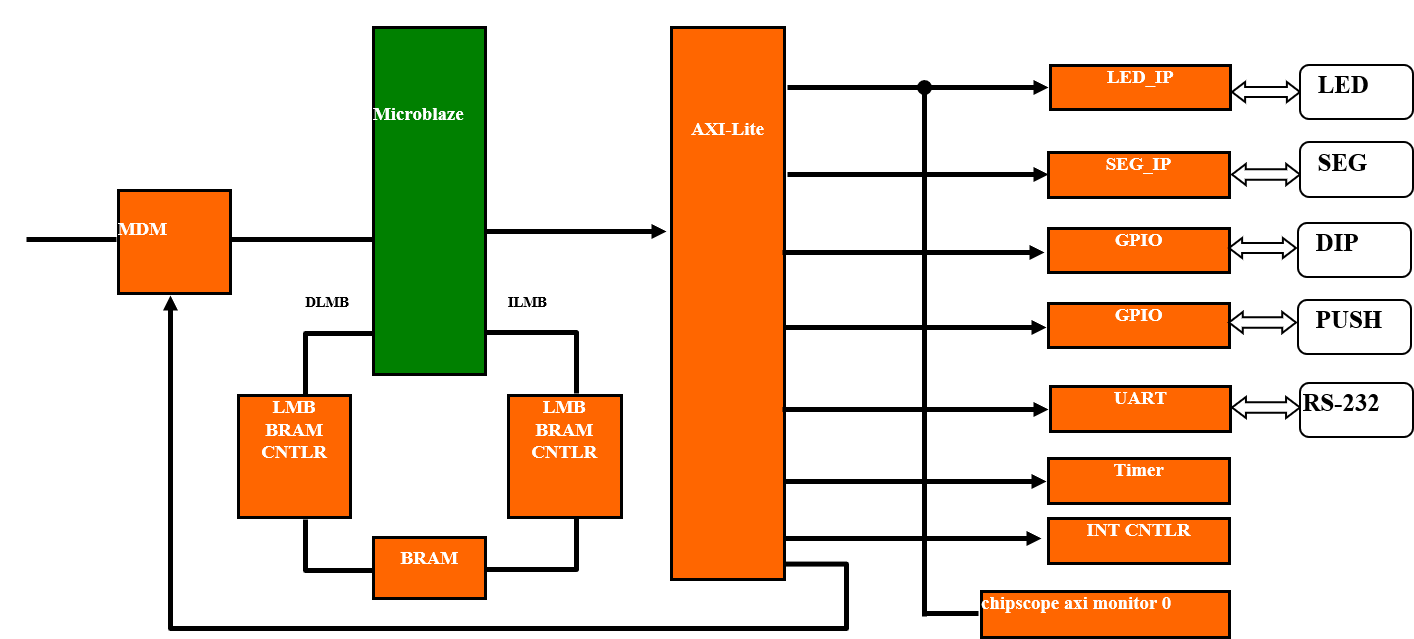
\includegraphics[width=1\linewidth]{report3-1}
\caption{系统完整结构}
\label{fig:report3-1}
        \end{figure}
        
        \begin{figure}[h!]
\centering
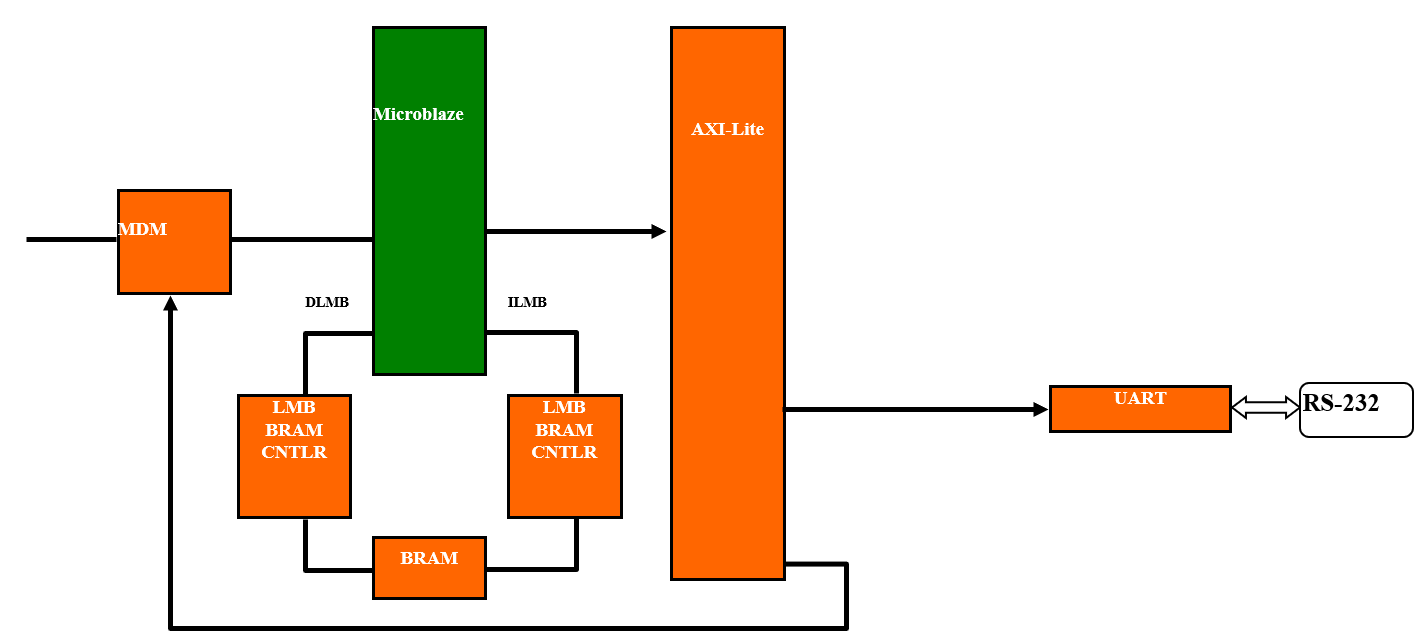
\includegraphics[width=1\linewidth]{report3-2}
\caption{实验内容}
\label{fig:report3-2}
        \end{figure}
        
        \paragraph{新建工程}
        
        在 XPS 通过 “Create New Project Using Base System Builer” 创建新的项目。
        
        在一个完整的路径中创建一个基于 AXI System 的系统。
        在提前安装好对 Digilent 的 Nexys 3 的板级支持包之后,
        配置我们的开发板。
        
        将 \verb|Local Memory Size| 设置为 16KB,
        并将除串口通信以外的所有外设移除。并点击 Finish
        结束向导。
        
        \subsubsection{添加 IP 核}
        
        由于本实验未设置其他内容,故不需要添加 IP 核。
        
        \subsubsection{配置 SDK}
        
        在正式配置 SDK 之前,需要依次通过 
        \verb|Generate Netlist| 与 \verb|Generate Bitstream|
        生成网表与比特流文件。
        
        然后在 \verb|Project -> Export Hardware ...| 选项中
        到处对于硬件的设计支持的 SDK。
        在弹出的对话框中,选择 \verb|Export \& Launch SDK|,
        并在 SDK 打开之后将工作空间定位到工程中的
        \verb|SDK\SDK_Export| 目录下。
        
        然后在 \verb|File -> New| 菜单选项中选择 \verb|Other|
        然后在对话框中找见 \verb|Board Support Package|
        创建板级支持包。

        然后在向导中选择 \verb|standalone| 并创建板级支持包。
        然后还是在 \verb|File -> New| 菜单中选择 \verb|Application|
        创建 C语言 的 HelloWorld 工程,并选择之前创建的板级支持包。
        
        \subsubsection{编写软件}
        
        我们的 \verb|Hello World| 跨越过一堆坑之后,终于可以开始编写了。
        在代码中编写:
        
        \begin{lstlisting}[language=C,caption=]
#include <stdio.h>
#include "platform.h"

void print(char *str);

int main()
{
    init_platform();

    print("Hello World\n\r");
    print("I was created on an unsuspecting world.\n\r");
    cleanup_platform();

    return 0;
}
        \end{lstlisting}

        \subsubsection{配置上板}
        
        在代码保存之后,程序是自动编译的,因此至此所需要的文件基本都准备好了。
        
        \paragraph{链接串口}
        
        在之前设计硬件的部分是使用串口进行通信。在 Windows 上使用
        PuTTY这个软件进行与 FPGA 开发板的通行。对于 macOS 或者 Linux
        等 Unix类的系统则是使用 minicon 进行串口的链接。
        
        之前配置的是 波特率是 115200,则在配置中配置好。
        
        然后在JTAG 配置中,配置成 Diligent 的 USB。然后将
        
        
\end{document}